
In this subsection, we relate the free energy to the amplitudes between boundary states and give analytic results. 

We notice that there is only one apparent length scale in these diagrams -- the finite size $L$ for fidelity and imaginary time $\tau$ for the Loschmidt echo. These are the characteristic size of the corner at the tip of the slit. However, without regulators the conformal invariance can rescale both to $1$ by doing a dilation transformation, thus getting rid of their dependence. Therefore, regulators are necessary in keeping track of the scale dependence and also physically sensible considering the lattice realization of the systems. 

We thus add small semi-circles around the points where the boundary condition changing operator resides and then do a series of conformal mapping. 

For the fidelity case, the regulators as well as conformal mapping are depicted in Fig.~\ref{fig:fidel-map} 
\begin{figure}[h]
\centering
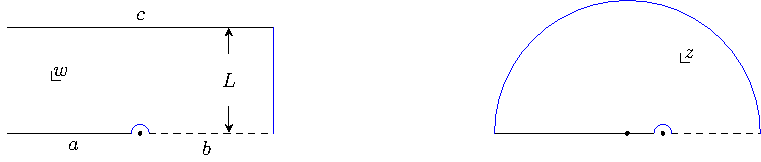
\includegraphics[width=\textwidth]{fig_fidel-map.pdf}
\caption{Mapping from a strip to the upper half plane $w = \frac{L}{\pi} \ln z $. The two black dots represent possible insertion of bcc operators. The dot inside the blue semi-circle is at coordinate $z = 1$, which is the image of point connecting $a$ and $b$ boundaries. The other dot is at $z = 0$, and corresponds to the connection between $a$ and $c$ boundaries at $- \infty$. To evaluate the diagram, we add the outer-semi-circle as the IR cut-off, it can also be regarded as the image of the blue vertical line on the $w$ plane.}
\label{fig:fidel-map}
\end{figure}
We assume $a = c$ such that there is only one bcc operator on the real axis enclosed by the regulator. The two end points of the $\epsilon$ radius semi-circle on the $w$ plane are mapped to
\begin{equation}
\exp( \pm \pi \frac{\epsilon}{ L}  ) \sim 1 \pm \pi \frac{\epsilon}{L} 
\end{equation}
The vertical line at $\text{Re} w = W$ (IR regulator) is mapped to $|z| = e^{\pi \frac{W}{L} } \gg 1 $. Since the radius of this larger circle is overwhelming, moving the inner semi-circle on the $z$ plane to the center will not affect the cross ratio to the leading order. The dashed line and solid line can then be regarded as two boundary states, the diagram corresponds to the following partition function
\begin{equation}
  Z_{ab} = \langle a | e^{-\pi H } |b \rangle 
\end{equation}



The Loschmidt echo can be evaluated the same way. Again we introduce two semi-circles (blue in Fig.~\ref{fig:H-tau_fold}) as regulator and then perform the conformal transformation shown in Fig.~\ref{fig:H-tau_fold}. In the $\xi$ plane, we end with the same diagram as fidelity. With one more conformal mapping, it is becomes the cylinder partition function between two boundary states. 

\begin{figure}[htb]
\centering
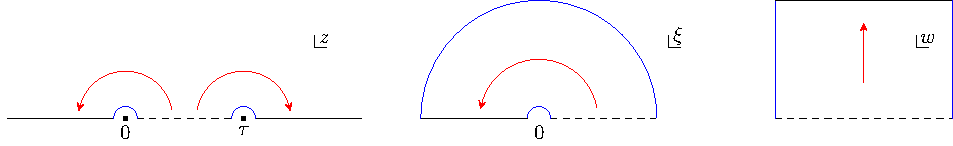
\includegraphics[width=\textwidth]{fig_H-tau_fold}
\caption{Left: diagram of the partition function of Loschimidt echo, where time is the horizontal direction, the dashed(solid) lines are open(gluing) boundary conditions. Red arrows are the directions of Hamiltonian flow that propagates the dashed line boundary state to the solid line boundary state. The blue semi-circles are UV regulators and they are identified as periodic boundaries in the direction perpendicular to the red arrow(equal time slice). Middle: image of the map $\xi = \frac{z}{\tau - z}$. Right: image of $w = \ln \xi$. It is a cylinder by identifying the blue lines and standard radial quantization can be applied. }
\label{fig:H-tau_fold}
\end{figure}

The results of the general partition function $S_a( \theta_1 ) \rightarrow S_b( \theta_2)$ and its free energy are evaluated in App.~\ref{app:lambda_12} to the leading order of cylinder width $\beta$. But one can't use these results na\"ively as we have tacitly introduced shifts in doing these conformal transformation. In fact, directly using the free energy given in App.~\ref{app:lambda_12} resulting in a power law increase of Loschmidt echo, which does not agree with the known results. One easy way to see the shift is that free energy is zero when $a,b,c$ are all periodic boundary conditions, hence 
\begin{equation}
\mathcal{F} = - \ln Z_{ab} ( \beta ) + \frac{1}{12} \beta 
\end{equation}
where $\frac{1}{12}\beta$ is the value of $ \ln Z_{ab} ( \beta )$ when $a = b = {\rm P}$. A more careful inspection is performed in App.~\ref{app:F_correction}, where the correction is found to be coming from the Schwartzian and outer circle regulator. 

For the process ($c$ is assumed to be the same as $a$)
\begin{equation}
S_i( \theta_1 ) \rightarrow S_j( \theta_2 ) 
\end{equation}
the free energy is
\begin{equation}
\mathcal{F}( \beta )  = 
\left\lbrace
\begin{aligned}
  &\frac{1}{2}(|x| - x^2 )\beta  \quad &i = j \\
  &\frac{1}{16}\beta   \quad &i \ne j   \\
\end{aligned} \right. \quad x = \frac{\theta_2 - \theta_1}{\pi} 
\end{equation}
We can then read off the fidelity and Loschmidt echo power law decay exponent with the identification $\beta = 2 \ln L$ and $ 4 \ln \tau$. 

As analyzed in Sec.~\ref{sec:analytic_numerics}, $S_2( \theta)$ interpolates between DD and NN, $S_1( \theta )$ interpolates between DN and ND. In the region accessible to the numerical calculation in the lattice model, we choose the process 
\begin{equation}
{\rm DD} + {\rm DD} \rightarrow  \lambda + {\rm DD}
\end{equation}
to verify
\begin{equation}
\mathcal{F} = 
\left\lbrace
\begin{aligned}
\frac{1}{8}\ln L  &\quad\text{fidelity}  \\
\frac{1}{4}\ln t   &\quad \text{echo}   \\
\end{aligned} \right.  
\end{equation}
where same results have already been obtained for $\lambda = {\rm P}$\cite{stephan_logarithmic_2013,stephan_local_2011,vasseur_universal_2014,vasseur_crossover_2013,kennes_universal_2014}. Another process
\begin{equation}
{\rm DN} + {\rm DN} \rightarrow \lambda + {\rm DN} 
\end{equation}
is used to verify
\begin{equation}
\mathcal{F} = 
\left\lbrace
\begin{aligned}
 (x - x^2 )\ln L   &  \quad {\rm fidelity} \\
 2(x - x^2 ) \ln t  & \quad \text{ Loschmidt echo} \\
\end{aligned} \right. 
\end{equation}
where $\lambda = \tan \theta$ and $x = \frac{\theta}{\pi}$. 

%%% Local Variables:
%%% TeX-master: "bCFT_paper"
%%% TeX-PDF-mode: t
%%% End:
